\documentclass[border=3pt]{standalone}
\usepackage{tikz}
\usetikzlibrary{arrows.meta,calc,positioning}
\tikzset{pin/.style={-{Stealth[length=5pt]}},
  bus/.style={{Stealth[length=5pt]}-{Stealth[length=5pt]}, thick},
  blk/.style={draw, thick, minimum width=22mm, minimum height=12mm, font=\sffamily\small, align=center}}
\begin{document}
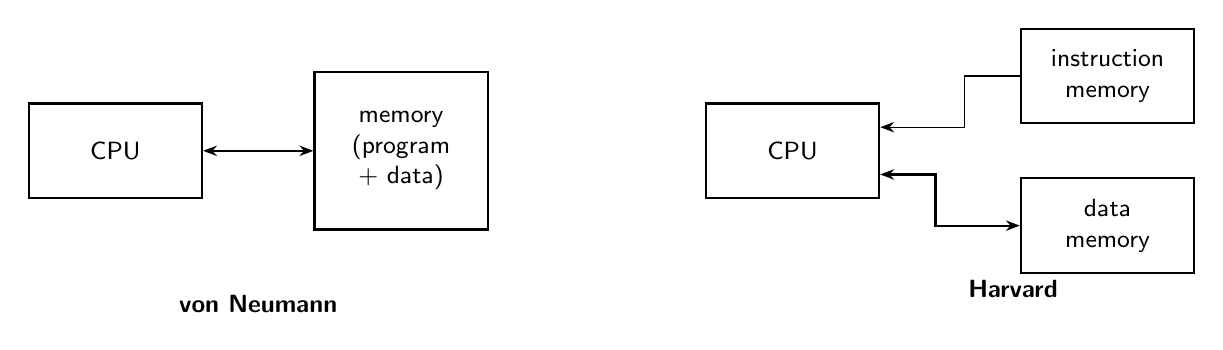
\begin{tikzpicture}[font=\sffamily\small]
  % von Neumann
  \node[blk] (cpu1) at (0,0) {CPU};
  \node[blk, right=14mm of cpu1, minimum height=20mm] (mem1) {memory\\(program\\+ data)};
  \draw[bus] (cpu1.east) -- (mem1.west);
  \node[font=\sffamily\small\bfseries, below=9mm of $(cpu1.south)!0.5!(mem1.south)$] {von Neumann};
  % Harvard
  \node[blk] (cpu2) at (8.6,0) {CPU};
  \node[blk] (imem) at (12.6,0.95) {instruction\\memory};
  \node[blk] (dmem) at (12.6,-0.95) {data\\memory};
  \draw[pin] (imem.west) -- ++(-7mm,0) |- ($(cpu2.east)+(0,3mm)$);
  \draw[bus] ($(cpu2.east)+(0,-3mm)$) -- ++(7mm,0) |- (dmem.west);
  \node[font=\sffamily\small\bfseries, below=9mm of $(cpu2.south)!0.7!(dmem.south |- cpu2.south)$] {Harvard};
\end{tikzpicture}
\end{document}
